\documentclass[12pt] {article}
\usepackage{enumerate}
\usepackage{algorithm2e}
\usepackage{mcode}
\usepackage{listings}
\usepackage{graphicx}
\usepackage{epsf}

\author{Zhengwu Zhang}
\title{Homework 3}

\begin{document} 
\maketitle
\newpage
\subsection{Problem 1}
(a) See figure 1
\begin{figure}
\begin{center}
\begin{tabular}{cc}
\includegraphics[height=2.1in]{prob1f0.eps}&
\includegraphics[height=2.1in]{prob1f.eps}\\
(a) & (b)
\end{tabular}
\caption{(a)Function of $x^2|sin(\pi x)|e^{-x^3}$. This implies that we could integrate the function from 0 to 3 (b) Density function of $f(x)$}
\end{center}
\end{figure}

(b) See figure 2
\begin{figure}
\begin{center}
\includegraphics[height=2.2in]{prob1hist.eps}
\caption{Histogram of Markov chain and $f(x)$}
\end{center}
\end{figure}

(c) $E(x)$= 0.8616 $var(x)$=  0.1417

Matlab Code:
\begin{lstlisting}
%homework 3
% we are going to use exponential distribution as proposal denstiy

f0=inline('x.^2.*abs(sin(pi*x)).*exp(-x.^3)','x');

c=quad(f0,0,4); 

f=inline('x.^2.*abs(sin(pi*x)).*exp(-x.^3)/c','x','c');

%q function

t=0:0.1:5;
%plot the density function of f(x);
plot(t,f(t,c));

% the M-H algorithm
K=5000;
x=zeros(1,K);
x(1)=0.5;

for k=2:K
    y=exprnd(1);
    rho=min((f(y,c)*exp(-x(k-1)))/(f(x(k-1),c)*exp(-y)),1);
    U=rand;
    x(k)=y*(U<rho) + x(k-1)*(U>rho);
end;

%compute histogram

h=histc(x,t)/K;

figure(2);
bar(t,h);hold on;
plot(t,f(t,c)/sum(f(t,c)),'m','linewidth',3);
ex=mean(x);
varx=var(x);
\end{lstlisting}

\subsection{Problem 2}
Solutions:
$\rho(x,y)=\frac{f(y)*q(x)}{f(x)*q(y)}$=$\frac{f_{Y|X}(6|y)*f_x(y)*q(x)/f(6)}{f_{Y|X}(6|x)*f_x(x)*q(y)/f(6)}$=$\frac{f_{Y|X(6|y)}}{f_{Y|X}(6|x)}$;

The target density function $f_{X|Y}(x|y)$ when $y=6$ is $f_{X|Y}(x|6)=\frac{e^{-|x-6|^{0.5}-(x-5)^2/8}}{\int{e^{-|x-6|^{0.5}-(x-5)^2/8}}}$
(1) Sample from the posterior for $y=6$;

\begin{figure}
\begin{center}
\begin{tabular}{ccc}
\includegraphics[height=1.1in]{st1_abr.eps}&
\includegraphics[height=1.1in]{st1_all.eps}&
\includegraphics[height=1.1in]{st1_50.eps}\\
(a) & (b) & (c)\\
\includegraphics[height=1.1in]{st6_bar.eps}&
\includegraphics[height=1.1in]{st6_all.eps}&
\includegraphics[height=1.1in]{st6_50.eps}\\
(a) & (b) & (c)
\end{tabular}
\caption{Top: (a)Sample from Posterior and original density function(Initial x=1).(b)5000 steps Evolution of the Chain (c) First 50 Steps Evolution; Bottom: Initial x=6}

\end{center}
\end{figure}

(2) Use the Markov chain to estimate the posterior mean and variance
Initial $x=1$:

$E(x)$ =

    5.4595


$Variance(x)$ =

    2.2726

Initial $x=6$:
$E(x)$ =

    5.4579


$Variance(x)$ =

    2.3152
    
    
Matlab Code:
\begin{lstlisting}
%homework 3
% Problem 2

f=inline('exp(-abs(x-6).^0.5)','x');

f0=inline('exp(-abs(x-6).^0.5-(x-5).^2./8)','x');

c=quad(f0,-2,14);

f1=inline('exp(-abs(x-6).^0.5-(x-5).^2./8)/c','x','c');
% the M-H algorithm
K=5000;
x=zeros(1,K);
x(1)=6;
t=-2:0.1:15;

for k=2:K
    y=5+2*randn(1); %nomal distribution with mu=5, var=4;
    rho=min(f(y)/f(x(k-1)),1);
    U=rand;
    x(k)=y*(U<rho) + x(k-1)*(U>rho);
end;

%compute histogram

h=histc(x,t)/K;

figure(2);
hold on; bar(t,h);hold on;
plot(t,f1(t,c)/sum(f1(t,c)),'b','linewidth',3);

ex=mean(x);
varx=var(x);

\end{lstlisting}

\end{document}